\section{Pianificazione} \label{sec:pianificazione}
In questa sezione viene riportato un diagramma di Gantt riassuntivo della pianificazione del lavoro nel periodo di stage. Come si può vedere le ore sono state suddivise secondo 4 obiettivi, che rappresentano parti di sistema indipendenti che verranno sviluppate in maniera autonoma. \\ \\
Come si può riscontrare nelle attività riportate nel diagramma lo svolgimento dello sviluppo non seguirà un classico modello a cascata. E' infatti previsto che dopo una prima parte di analisi generale del sistema (che servirà a comprendere le relazioni tra le varie parti e le caratteristiche e funzionalità del software nella sua interezza), l'implementazione concreta delle varie parti avvenga secondo un modello che prevede la suddivisione del lavoro in piccoli incrementi. Ciò è reso possibile dalla completa indipendenza delle varie parti in cui il core è stato suddiviso. Il modello di ciclo di vita utilizzato può essere paragonato ad uno \textit{scrum}: è infatti emerso nei primi tempi che tale modello era preferibile rispetto alla rigidità dei modelli più classici, in quanto permetteva lo sviluppo continuo dei vari incrementi e la possibilità di mostrare passo per passo i risultati ottenuti. Per chiarezza si riporta una breve descrizione degli obiettivi presenti nel piano di lavoro che verranno maggiormente approfonditi nelle sezioni successive:
\begin{description}
	\item \textbf{Obiettivo 1} Generazione di un \textit{heatmap} a partire dall'input di un file .DXF che descrive la planimetria del locale e da un file .CSV che contiene una lista di coordinate di tracciamento
	\item \textbf{Obiettivo 2} Realizzazione di un tool per la calibrazione delle telecamere
	\item \textbf{Obiettivo 3} Integrazione nel core di una base di dati per la consistenza dei dati e delle configurazioni
	\item \textbf{Obiettivo 4} Recupero di informazioni statistiche significative a partire dai dati di tracciamento
	
\end{description}

In figura ~\ref{fig:pianificazione} è presente il diagramma di Gantt di cui sopra. Le voci del menù che portano la voce verifica sono da intendersi come ore dedicate all'esecuzione dei test precedentemente definiti.
\begin{figure}[!t]
\centering
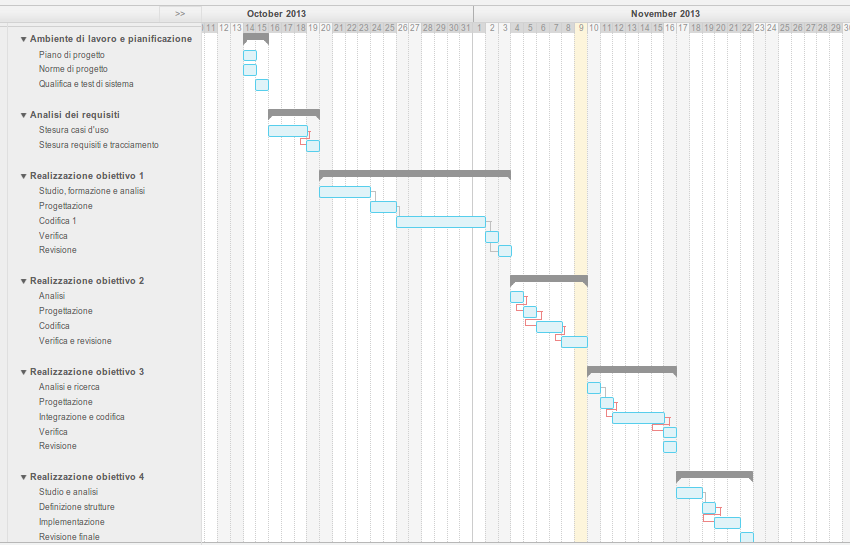
\includegraphics[width=1.0\textwidth]{./images/pianificazione.png}
\caption{diagramma di Gantt che descrive la pianificazione}
\label{fig:pianificazione}
\end{figure}






